\documentclass[a4paper]{article}
\usepackage[utf8]{inputenc}
\usepackage{amsmath}
\usepackage{graphicx}
\usepackage[procnames]{listings}
\usepackage{color}
\usepackage{indentfirst}
\usepackage{xcolor}
\usepackage{sectsty}
\usepackage[explicit]{titlesec}
\usepackage[hidelinks]{hyperref}

\usepackage[normalem]{ulem}
\usepackage{geometry}
 \geometry{
 a4paper,
 %total={170mm,257mm},
 left=20mm,
 %top=20mm,
 }
\title{\textbf{ SA/SD Document}}

\author{}
\date{}

\begin{document}


\maketitle
\begin{center}

\includegraphics[scale=0.6]{images/logoLIS_modified.jpg}
\\
\textbf{LIBRERIA}\\
LIBRARY INFORMATION SYSTEM\\
%\vspace{2 cm}
Group Number : 52\\
Group members: \\
\begin{itemize}
\item \begin{center}Ashrujit Ghoshal (14CS10060)\end{center}
\item \begin{center}Sayan Ghosh (14CS10061)\end{center}
\end{itemize}

\end{center}
\newpage
%\clearpage
\hypertarget{toc}{}
\tableofcontents
\newpage
\part{System Analysis}
\section{Feasibility Study}
\subsection{Understanding the problem}
In this section, we make an effort to understand the purpose of the software.
\\
The LIS(Library Information Software) is intended to ensure a systematic manner of maintaining the database of a library and easing the job of a librarian.The LIS will help maintain a record of books in the library and members registered with the library.The software aims at hassle-free handling of basic library functions like issue/reserve/return books as well as giving the freedom to the librarian to add and delete books and members to the database.
	Extending further the software can be used by the librarian to decide on disposing of books which have not been issued for a long time. This software also helps to keep track of statistics of issue of a particular book ver a period of time.Since everything is done on the computer, it is easy to record all data and there are minimal chances of inconsistencies or ambiguities.
Also use of a secure database support enhances the security aspects of the software thus enabling to create a more robust and secure software
\subsection{Scope of the Problem}
In this section,we list the various functions performed by the software:
\begin{itemize}
\item Add books to the database
\item Modify existing records of books
\item Delete unused books from database
\item Add users to the database
\item Modify existing details of users
\item Remove user from the database
\item Query regarding books on ISBN nnumber or name
\item Query regarding user on user id or name
\item Record issue,return and reservation of books
\item Calculation of penalty on overdue books
\item Maintainence of statistics of all books 
\end{itemize}
\subsection{Analysing stakeholders}
The various stakeholders are:
\begin{itemize}
\item Librarian
\item Library Clerk
\item Member / Library user
	\begin{itemize}
	\item Faculty
	\item Research Scholar
	\item PG Student
	\item UG Student
	\end{itemize}
\end{itemize}
These stakeholders have been clearly described with their attributes and methods in the SRS.
\subsection{Defining Alternatives}
\subsubsection{Connection between software and librarian}
The librarian is treated as the administrator of the software who has the sole capability to create and delete the members like the faculty or the students (including research scholars,UG and PG students).
\\The librarian can  send a print notification if required if a penalty is required to be paid in case of overdue of a book
\\Also the librarian can study the book statistics and can send a notification to the clerk to dispose off old and unused books from the library database
\subsubsection{Connection between software and member}
The members can perform the following operations:
\begin{itemize}
\item Can issue a book if available in the library
\item Can request for reserving a book if already issued to another user (subjected to the condition that he does not exceed his/her maximum book limit)
\item Can return a book to the library
\item pay fine/penalty if required in case of a overdue of book
\end{itemize}
\subsubsection{Hardware Infrastructure}
\begin {enumerate}
	\item Processor Pentium II processor or higher
	\item Hard Disk space 500MB
	\item RAM 512 MB
	\item Network/Internet accesss
\end{enumerate}
\subsubsection{Software Infrastructure}
\begin{enumerate}
	\item Operating system
		\begin{itemize}
		\item  Windows 7 or later
		\item Linux distributions like Ubuntu 14.04.03 or other
		\end{itemize}
	\item MySQL
	\item Java JDK platform 1.7 or higher
	\end{enumerate}
\subsubsection{Technology Used}
The technologies used are as follows :
\begin{itemize}
\item Use of the platform independent JVM using JDK 1.8
\item MySQL support to provide DBMS features to the software
\end{itemize}
\subsubsection{Security}
The security of the software has been taken care of in a very cautious and judicious manner. The protocol followed to ensure data security and software safety are as follows :
\begin{itemize}
\item User can accesss the books only after a successful login with a valid username and password.
\item Check has been done during creation of new user to ensure a unique user id.
\item Also check has been done to set a minimum length of 8 characters and use of alphanumeric characters to make a password without storing any value (to prevent publicity of password) so that users can give a safe and efficient password to safeguard their account. 
\item Unsuccessful attempts may occur if the user gives wrong username or wrong password or even wrong user type.
\end{itemize}
\subsection{Defining Criteria to evaluate}
The software is evaluated on the basis of the following criterias:
\begin{itemize}
\item Only the librarian can be created without any preprocessing. But only one librarian must be present.
\item Addition and deletion of books can be performed by library clerk in this software
\item Creation of users by the librarian can be performed effectively
\item Users should be able to successfully login into the software
\item Creation of effective users who can perform all the operations like issue, reserve and returning of a book
\end{itemize}
\subsection{Report}
The software designed is able to perform all the above operations mentioned above. One can create a single librarian at first when hold the admin accesss of the software.The librarian is able to create the users or the library members who can perform all the required operations as mentioned in the SRS.
\\The library clerk is able to add books into the library and can remove the unrequired books from the database.
\\The login feature has also been created,tested and is working perfectly.Only the authenticated users can log into the software to perform the designated operations.
\\A background cron job takes care of all the background processes and helps to maintain all the records as required like in the case of issuing and returning.It also takes care of the issued books and takes care if a penalty is to be issued against any user account.
\\All the process as mentioned in the SRS document provided have been implemented and tested successfully.

\section{UML Diagrams}

\subsection{Refinement of Use Case Diagram}

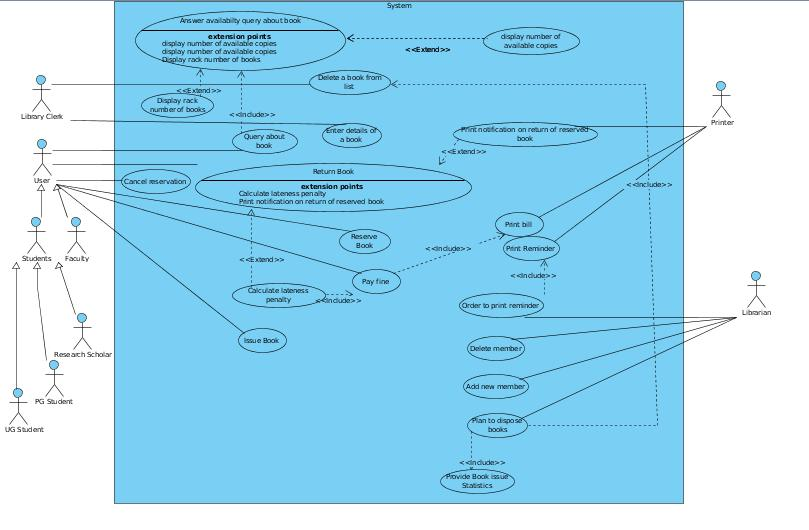
\includegraphics[scale=0.55]{images/useCaseDiag.jpg}\\

Description :
\\
\begin{enumerate}
\item User use cases:
	\begin{itemize}
	
	\item Query about Book\\
	\begin{itemize}
	\item Preconditions:\\
	1. The user must be logged in .\\
	2.The book must exist in the library\\
\item  Postcondition: \\If the book exists in the library,the availability status of the book is returned\\
 \item Failure Situations:\\ The library does not have  the book \\
 \item Postcondition in case of failure:\\A message to user about the same\\
\item  Actors:\\ User communicates with the system\\
\item  Trigger:\\ User chooses the option to search books\\
 \item Main Success Scenario: \\The library has a copy of the book and it is available for issue.\\
\item  Extensions/Variations: \\The library has a copy of the book but currently none of the copies are available.The book maybe reserved by the user.
	\end{itemize}
 \item Issue Book\\
	\begin{itemize}
	 \item Preconditions:\\
	 1. The user must be logged in .\\
	 2.The book must exist in the library \\
	 3.It must be available for issue.\\
	 4.The user must not have exhausted his quota of nnumber of books\\
 \item Postcondition:\\After successful issue the user account is updated\\
 \item Failure Situations:\\
 1. The library does not have  the book\\ 
 2.The library has the book and it is not available for issue.\\
 3.The user has exhausted his quota of maximum nnumber of books\\
 \item Postcondition in case of failure:\\In failure case 2. the user may choose to reserve the book if he has not exhausted his quota\\
 \item Actors:\\ User communicates with the system\\
 \item Trigger: \\User chooses the option to issue books\\
 \item Main Success Scenario:\\ The library has a copy of the book and it is available for issue.
	\end{itemize}
 

 \item Return Book\\
 \begin{itemize}
 \item Precondition:\\
 1.User must be logged in.\\
 2.User must have previously issued the book.\\
 \item Postcondition:\\
 1.If the book was overdue the penalty is calculated and a bill is printed\\ 
 2.In case the book was reserved by some other user, a notification is sent out to the other user.\\
 3.The user account is updated\\
 \item Failure Situations:\\The user has not issued any book\\
 \item Postcondition in case of failure:\\A message is give to the user about the same\\
 \item Actors:\\ User communicates with the system\\
 \item Trigger:\\ User chooses the option to return issued books\\
\item  Main Success Scenario: \\The user had previously issued the book\\
 \end{itemize}
 
 \item Reserve Book\\
	\begin{itemize}
	\item  Preconditions:\\
	1. The user must be logged in .\\
	2.The book must exist in the library\\ 
	3.It must not  be available for issue.\\
	4.The user must not have exhausted his quota of nnumber of books\\
 \item Postcondition:\\
 1.After successful issue the user account is updated \\
 2.When the book is returned a notification is sent to the user.\\
 \item Failure Situations:\\
 1. The library does not have  the book \\
 2.The library has the book and it is  available for issue.\\
 3.The user has exhausted his quota of maximum nnumber of books\\
 \item Postcondition in case of failure:\\In failure case 2. the user may choose to issue the book if he has not exhausted his quota\\
 \item Actors:\\ User communicates with the system\\
 \item Trigger:\\ User chooses the option to reserve book\\
 \item Main Success Scenario:\\ The library has a copy of the book and it is not available for issue.\\
 
	\end{itemize}
 
 \item Cancel Reservation\\
 \begin{itemize}
 \item  Preconditions:\\
 1. The user must be logged in .\\
 2.The user must have reserved the book\\
 \item Postcondition:\\
 1.After successful issue the user account is updated \\
Failure Situations:\\The user has not issued any book\\
 \item Actors: \\User communicates with the system\\
 \item Trigger:\\ 
 1.User chooses the option to cancel reservation of a book \\
 2.User does not issue the reserved book within 7 days of return\\
 \item Main Success Scenario:\\ The library has a copy of the book and the user must have reserved it previously\\
	
 \end{itemize}

\item Pay Fine\\
	\begin{itemize}
	\item  Precondition:\\
	\begin{enumerate}	
	\item User must be logged in.\\
	\item User must have previously issued the book.\\The book must be overdue\\
	\end{enumerate}
 \item Postcondition:\\
  The book was overdue the penalty is calculated and a bill is printed 
 \item Failure Situations:
 \begin{enumerate}
 \item The user has not issued any book
  \item No returned books are overdue
	\end{enumerate} 
 \item Actors: User communicates with the system
 \item Trigger: User chooses the option to return issued books
 \item Main Success Scenario: The user had previously issued the book and the book is overdue
	\end{itemize}
\end{itemize}


\item Library Clerk Use Cases
 \begin{itemize}
 \item Enter details of a book
 \begin{itemize}
 \item Preconditions:1. The clerk must be logged in.\\2.The book must not be previously entered in the system
 \item Failure Situations:\\ The book is already in the system
 \item Postcondition in case of failure:\\A message to clerk about the same
 \item Actors:\\ library clerk communicates with the system
 \item Trigger:\\ Clerk chooses the option to enter new books
 \item Main Success Scenario:\\ The library  does not have the book and the book is newly entered in the system
\item  Extensions/Variations:\\ The library has the book and the number of copies is increased
\end{itemize}
 \item Delete a book 
 \begin{itemize}
	\item 	Preconditions:\\1. The clerk must be logged in.\\2.The book must  be previously entered in the system \\3.The librarian has decided to dispose the book\\
 \item Failure Situations:\\ The book is not in the system\\
 \item Postcondition in case of failure:\\A message to clerk about the same\\
 \item Actors:\\ library clerk communicates with the system\\
 \item Trigger:\\ Clerk chooses the option to delete books\\
 \item Main Success Scenario:\\ The library  has the book and it is removed from the system.\\
 \item Extensions/Variations: \\The library has the book and the nnumber of copies is reduced.\\
 
\end{itemize}	 
 
 \end{itemize}
 


\item Librarian Use Cases:
\begin{itemize}
 \item Add new member
 \begin{itemize}
  \item Preconditions:1.Librarian must be logged in\\2. A person must apply for membership
 \\ \item Postcondition:\\A new member account is created \\
 \item Failure Situations:\\ The user is already registered\\
 \item Postcondition in case of failure:\\A message to librarian about the same\\
\item  Actors:\\ Librarian communicates with the system\\
 \item Trigger: \\Librarian  chooses the option to add member\\
 \item Main Success Scenario:\\ The user is not previously registered\\
 \end{itemize}

\item Delete member\\ 
 \begin{itemize}
  \item Preconditions:\\ 1.Librarian must be logged in\\ 2. A person must apply for cancellation membership\\ 
 \item Postcondition:\\ The member account is deleted\\ 
 \item Failure Situations: \\ The user has no account\\ 
 \item Postcondition in case of failure:\\ A message to librarian about the same\\ 
 \item Actors: \\ Librarian communicates with the system\\ 
 \item Trigger:\\  Librarian  chooses the option to delete member\\ 
 \item Main Success Scenario:\\  The user   previously has an account\\ 
 \end{itemize}
 
 \item Order to print reminder\\ 
 \begin{itemize}
  \item Preconditions:\\ 1.Librarian must be logged in\\ 2. A book issued by a member must be overdue\\ 
 \item Postcondition:\\ A message is sent to the user.\\ 
 \item Failure Situations:\\  There are no overdue books\\ 
 \item Postcondition in case of failure:\\ A message to librarian about the same\\ 
 \item Actors: \\ Librarian communicates with the system\\ 
 \item Trigger:\\  Librarian  chooses the option to print reminder\\ 
 \item Main Success Scenario :\\  There are some overdue books\\ 
 \end{itemize}

\item Plan to dispose books\\ 
 \begin{itemize}
  \item Preconditions:\\ 1.Librarian must be logged in\\ 2. The book must not have been issued even once for 5 years\\ 
 \item Postcondition:\\ The book is disposed with a message to the library clerk to delete it.\\ 
 \item Actors:\\  Librarian communicates with the system\\ 
 \item Trigger:\\  Librarian  chooses the option to dispose book\\ 
 \item Main Success Scenario:\\  The book has not been issue for 5 years\\ 
 \end{itemize}
 

\end{itemize}

\item System Use Cases:\\ 
 \begin{itemize}
 
  \item Answer availability Query about Book\\ 
	\begin{itemize}
	\item  Preconditions:\\ 1.An user makes a query\\ 
 \item Postcondition: \\ If the book is available, use cases display rack nnumber and nnumber of copies are called\\ 
 \item Actors:\\  System communicates with the user\\ 
 \item Trigger: \\ User chooses the option to search books\\ 
	\end{itemize}

\item Display rack nnumber of book\\ 
	\begin{itemize}
	\item  Preconditions:\\ 1.If the book is available the use case answer availibility query invokes this\\ 
 \item Postcondition:\\  Rack nnumbers are displayed\\ 
 \item Actors:\\  System communicates with the user\\ 
 \item Trigger:\\  answer availibity query triggers this\\ 
	\end{itemize}
 
 \item Display nnumber of copies of book\\ 
	\begin{itemize}
	\item  Preconditions:\\ 1.If the book is available the use case answer availibility query invokes this\\ 
 \item Postcondition:\\  the nnumber of copies of a book are displayed\\ 
 \item Actors: \\ System communicates with the user\\ 
 \item Trigger:\\  answer availibity query triggers this\\ 
	\end{itemize}

\item Calculate lateness penalty\\ 
	\begin{itemize}
	\item  Preconditions:\\ 1.If the book is overdue, return book invokes this\\ 
 \item Postcondition:\\ Penalty is calculated and print bill is invoked\\ 
 \item Actors: \\ System communicates with the user\\ 
 \item Trigger: \\ return book query triggers this\\ 
	\end{itemize}
 
 \item Provide book issue statistics
	\begin{itemize}
	\item  Preconditions:\\ 1.The use case is invoked by plan to dispose books\\ 
 \item Postcondition:\\ Statistics of books is displayed\\ 
 \item Actors: \\ system communicates with librarian\\ 
 \item Trigger:\\ Plan dispose book is invoked\\ 
	\end{itemize}

 \end{itemize}
\item Printer use cases:\\ 
\begin{itemize}
\item Print bill of penalty\\ 
\begin{itemize}
\item Preconditions:\\ Some user must have returned the issued book later than his designated return date.\\ 
 \item Postcondition:\\ Bill of penalty is printed\\ 
 \item Actors:\\  Printer communicates with the system\\ 
 \item Trigger:\\  Calculate lateness penalty triggers print bill\\ 
\end{itemize}

\item Print reminder\\ 
\begin{itemize}
\item  Preconditions:\\ Some user must have exceeded the due date\\ 
 \item Postcondition:\\ Reminder to user is printed\\ 
 \item Actors:\\  Printer communicates with the system\\ 
 \item Trigger:\\ order to print reminder triggers this\\ 
\end{itemize}

\item Print notification on return of reserved book\\ 
\begin{itemize}
\item Preconditions:\\ Some user must have returned a reserved book \\ 
 \item Postcondition:\\ A notification is printed to the user who reserved the book\\ 
 \item Actors: \\ Printer communicates with the system which communicates with user\\ 
 \item Trigger:\\ return book may trigger this use case\\ 
\end{itemize}

\end{itemize}
\end{enumerate}

\subsection{Refinement of Class Diagrams}
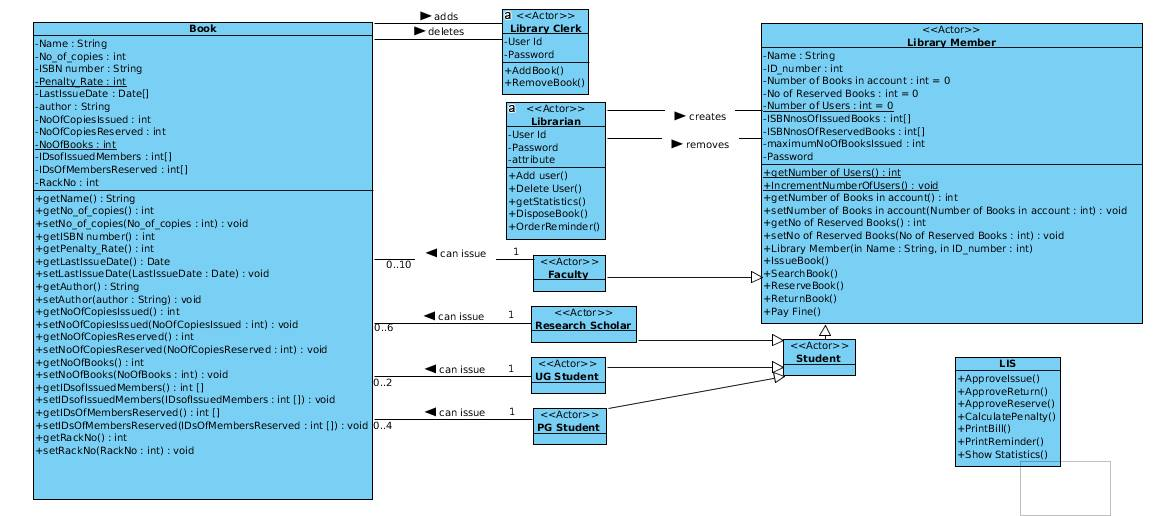
\includegraphics[scale=0.35]{images/classDiagFinal.jpg}
\\
Description : \\

\begin{itemize}
\item Book
\begin{itemize}
\item Class Attributes:\\
\\Name:Store the name of book
\\No$\_$of$\_$copies:Stores the nnumber of copies of a book
\\Penalty$\_$Rate:the rate of penalty for book.A static member as it is common for all the books
\\Author:stores name  author of book 
\\LastIssueDateDate:Stores the last issued date of book
\\NoOfCopiesIssued:Stores the nnumber of copies of the book that have been issued out
\\NoOfCopiesReserved:Stores the nnumber of issued books that have been reserved
\\NoOfBooks:A static variable storing the total nnumber of books
\\IDsofIssuedMembers[]:An array of integers storing the ids of all the members who have issued copies of the book
\\IDsOfMembersReserved[]:An array of integers storing the ids of all the members who have issued copies of the book
\\RackNo:stores the rack nnumber where the book is kept

\item Operations:
\\Getter functions for name,No$\_$of$\_$copies,ISBN nnumber,Penalty$\_$rate,LastIssueDate,author,NoOfCopiesIssued,NoOfCopiesReserved,NoOfBooks,IDsofIssuedMembers,IDsOfMembersReserved,RackNo.

We have used getters for these as we need to view these attributes from outside 
\\
Setters for No$\_$of$\_$copies,LastIssueDate,NoOfCopiesIssued,NoOfCopiesReserved,IDsOfIssuedMembers, IDSOfMembersReserved,RackNo.

We have used setters for these as these are changeable with time and need to be changesd at a later point of time.These being private members setters ar only way to modify them
\end{itemize}


\item Library Member 
\begin{itemize}
\item Attributes:
\begin{itemize}
\item Name:Name of the user
\item ID$\_$nnumber:Login id of the user
\item Nnumber of books in account:Total nnumber of issued books
\item Nnumber of reserved books:Total nnumber of books issued by the user
\item NoOfUsers:A static variable storing total nnumber of users
\item ISBNnosOfIssuedBooks[]:an array storing the ISBN nnumber of all books issued by the user
\item ISBNnosOfReservedBooks[]:an array storing the ISBN nnumber of all books reserved by the user
\item maximumNoOfBooksIssued:the maximum nnumber of books that the user can issue
\item password:The login password of the user which is necessary for login authentication
\end{itemize}

\item Operations:
\begin{itemize}

\item Constructor to initialize member\\
\item Getters for NnumberOfBooksinAccount,No ofReservedBooks,NoOfUsers.
We have used getters for these as we need to view these attributes from outside \\\
\item Setters for NnumberOfUsers,Nnumber of books in account,No Of reserved Books.


We have used setters for these as these are changeable with time and need to be changesd at a later point of time.These being private members setters ar only way to modify them
\\
\item IssueBook:called when member tries to issue a book\\
\item SearchBook:Called when member tries to search fo a book\\
\item Reserve Book:Called when member tries to reserve a book\\
\item ReturnBook:called when member tries to return a book\\
\item PayFine:Called when member returns an overdue book\\

\end{itemize}
\end{itemize}

\item Library Clerk
\begin{itemize}
\item Attributes:
\begin{itemize}
\item UserId:User Id of the library Clerk\\
\item Password:Password of the library Clerk\\
\end{itemize}

\item Operations:
\begin{itemize}
\item AddBook:Adds a new procured book to database\\
\item Removebook:Deletes a disposed book from database\\
\end{itemize}
\end{itemize}
\item Librarian

\begin{itemize}

\item Attributes:
\begin{itemize}
\item UserId:User Id of the librarian
\item Password:Password of the librarian
\end{itemize}
\item Operations:
\begin{itemize}
\item AddUser:Adds a new user account
\item DeleteUser:Deletes an existing user account
\item getStatistics: asks for statistics from LIS
\item DisposeBooks:Disposes a book not issued in 5 years
\item OrderReminder:Orders LIS to print reminder on overdue books
\end{itemize}
\end{itemize}

\item LIS
\begin{itemize}
\item Operations:\\
\begin{itemize}

\item ApproveIssue:Called when user tries to issue a book
\item ApproveReturn:Called when user tries to return a book

\item ApproveReserve:Called when user tries to reserve a book
\item CalculatePenalty:Calculates penalty on overdue book
\item PrintBill:prints penalty Bill
\item PrintReminder:prints Reminder on overdue books
\item Show Statistics:Display statistics of books issued

\end{itemize}
\end{itemize}

\item Faculty\\
It is a generalization of Library User
\item Student\\
It is a generalization of Library User
\item Research Scholar\\
It is a generalization of Student
\item UG Student\\
It is a generalization of Student
\item PG Student\\
It is a generalization of Student

\end{itemize}
\subsection{Sequence Diagram}
\subsubsection*{Add User Sequence Diagram}
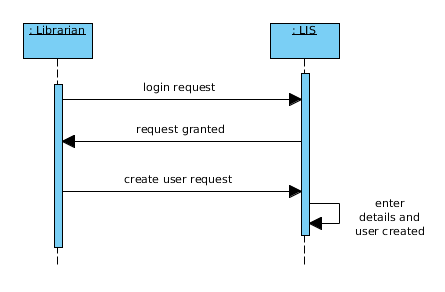
\includegraphics[scale=0.50]{images/seqDiagAddUser.png}
\\
Description : The user needs to login successfully into the account as the librarian as he/she only has the privilege to add a user .He then provides the suitable details required to create a user in the library and creates it.
\\

\subsubsection*{Remove User Sequence Diagram}
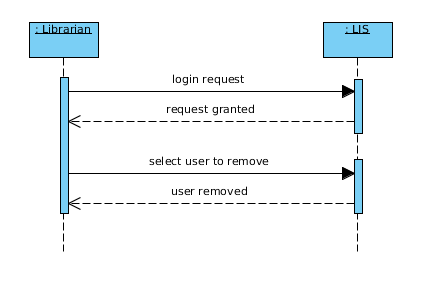
\includegraphics[scale=0.50]{images/seqDiagRemoveUser.png}
\\
Description : The user needs to login successfully into the account as the librarian as he/she only has the privilege to remove a user .He then provides the suitable details required to remove a user in the library and the user along with all the user history is removed from the library database.
\\

\subsubsection*{Add book Sequence Diagram}
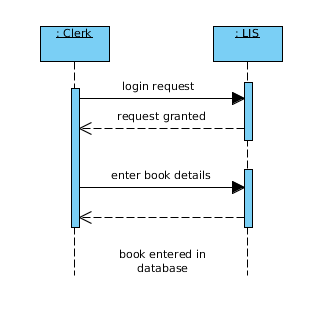
\includegraphics[scale=0.50]{images/seqDiagAddBook.png}
\\
Description : The user needs to login successfully into the account as the library clerk as he/she only has the privilege to add a book into the database of the library.The clerk then provides the suitable details of the book into the system and it automatically updates this into the database at the same time. The book will then be available for issuing ad reservation by the members.
\\

\subsubsection*{Remove book Sequence Diagram}
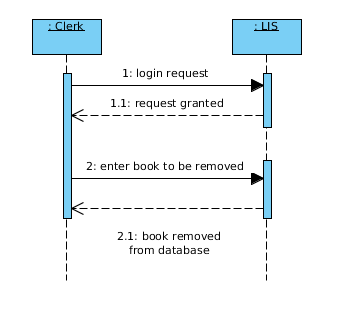
\includegraphics[scale=0.50]{images/seqDiagBookRemoval.png}
\\
The user needs to successfully login as the library clerk as he/she only has the privilege to remove a book from the system if he/she feels that the book has been unused for a long period of time and is not required anymore.The user feeds the details of the book to be removed and the system automatically removes all the records related to this book from the system and will not be thereafter available for issuing and reservation by the other library members/users.
\\

\subsubsection*{Issue book Sequence Diagram}
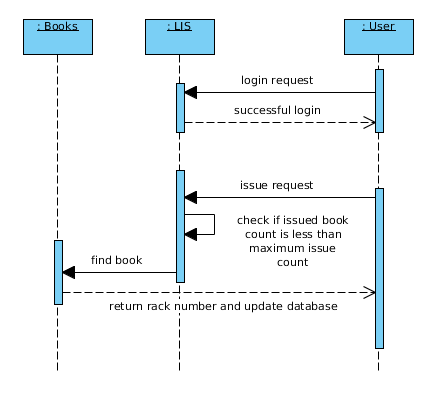
\includegraphics[scale=0.50]{images/seqDiagIssueBook.png}
\\
The user needs to successfully login as a valid member or user of the library to issue a book. Also the book must be available in the library at that instant and also he/she must not exceed the maximum book count against his/her account in the library.The book is then added into the user's account and is thus issued.\\

\subsubsection*{Return book Sequence Diagram}
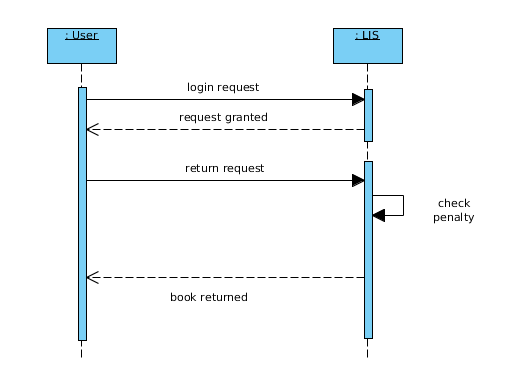
\includegraphics[scale=0.50]{images/seqDiagReturnBook.png}
\\
The user needs to successfully login as a valid member of the library to avail the option of returning the book.The book should not be overdue else the user has to pay a fine as per the rate predecided by the library authority. The book in any case is returned and all changes are updated in the user details of the database.
\\

\subsubsection*{Search book Sequence Diagram}
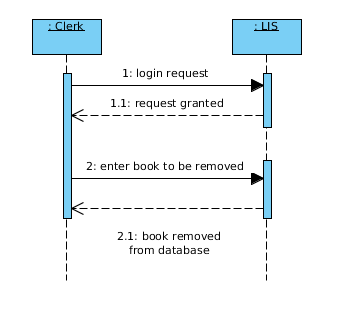
\includegraphics[scale=0.50]{images/seqDiagBookRemoval.png}
\\
The user needs to successfully login to search if a book is present in the library.The user needs to give the details of the book in the system and it will notify about the presence of the book in the library.
\\

\subsection{Collaboration Diagram}

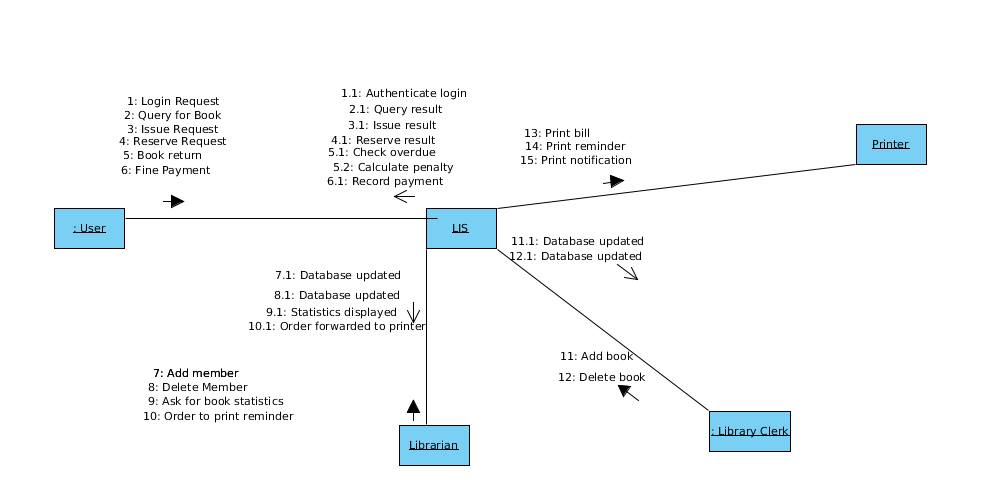
\includegraphics[scale=0.50]{images/collaDiag.jpg}
\\
Description : The user send a specific set of requests to the LIS system like the login request , issue request , return request , search request and penalty/fine payment.The LIS is bound to send back suitable return messages in case of each of the request messages sent ot the system.
\\
The library clerk has the privilege of adding and removing books from the system and the LIS system will automatically update its database inside by a cron job.
\\
The librarian has the sole administrator accesss to the software and the privilege of adding a member as well as removing his record from the library.The librarian can access the user details or the history of any user.He can also take a a look into the statistics of any book that is can see the book history and can send a notification to remove a book to the library clerk in case the book has been unused and unissued for a long period of time.
\\
The printer is also linked with the system and is used to print the notification and the penalty bills and reminder notifications

\subsection{Statechart Diagram}

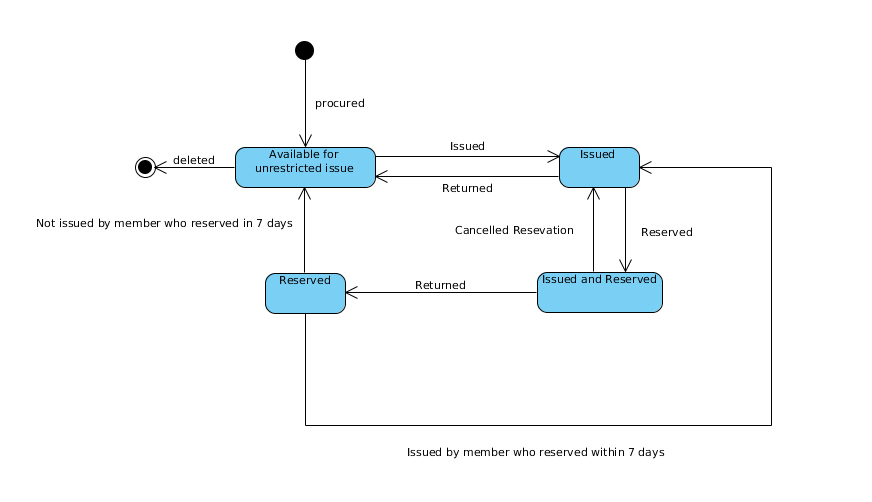
\includegraphics[scale=0.50]{images/stateDiagIssue.png}
\\
Description : The book is avilable for unrestricted issue if it has not been reserved or it has been then the user who has reserved it has not issued it within the 7 days after the notification that the book is available. The book is issued and returned in a separate state. There is also a facility to cancel a reservation .Even after issuing the book may be reserved by some other user. The transition between the states have been clearly shown and demarcated in the above diagram


\subsection{Activity Diagram}
\subsubsection*{Issue Book Activity Diagram}
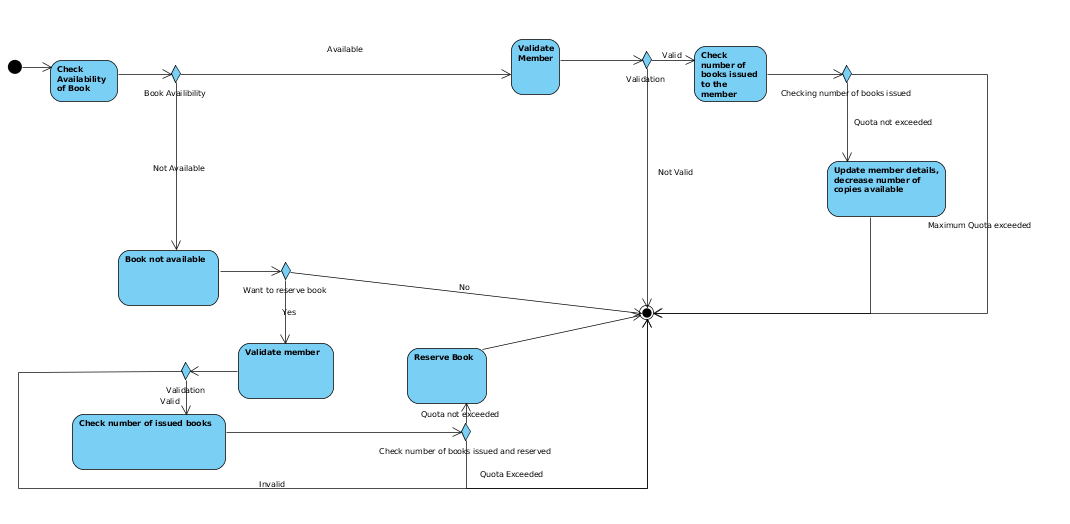
\includegraphics[scale=0.50]{images/activityDiagIssue.png}
\\
Description : First after succesful login the member has to check the availability of the book.We then check if the user is still allowed to issue books or if he has exceeded the maximum book count against his/her account.In case the book is avilable then the book is iisued and the required changes are made to his/her respective account. In case the book is not available then the user can decide to reserve the book or not.If he reserves the book then again we validate him and take a note of the reservation made.A notification will be made to him when the book will be available in the library
\subsubsection*{Return Book Activity Diagram}
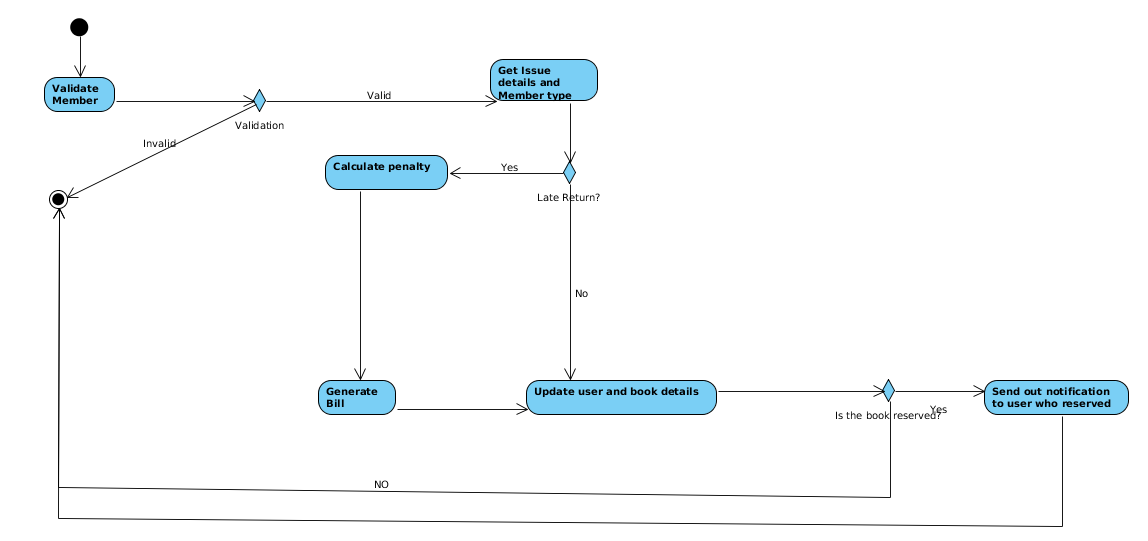
\includegraphics[scale=0.40]{images/activityDiagReturn.png}
\\
Description : We first check for the validation of the member. If the member successfully logs into his/her account then we ask for the book to be returned. The time for the issue is then checked and using that the nnumber of days he book has been kept is calculated. If trhe book has been kept for a longer period of time than it was meant to be the member or the user is liable to pay fines as per the rate predecided.The fine is calculated by a base on the time the book has been overdue.In any case the book is returned and required updation is donw on the account of the user.
\subsubsection*{Search Book Activity Diagram}
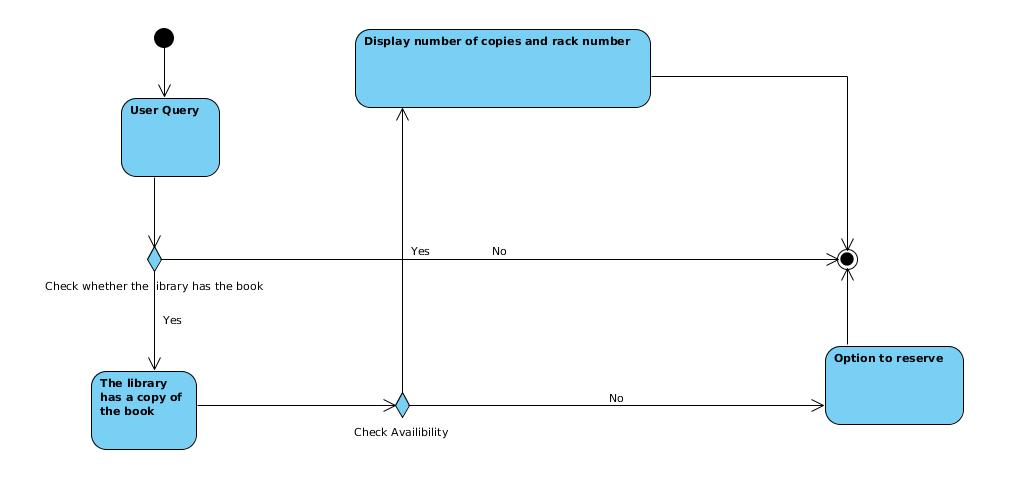
\includegraphics[scale=0.50]{images/activityDiagSearch.jpg}
\\
Description : The user may not need to validate into the system that is the search feature is kept as a global accesss feature. The person needs to put in the details of the book required in the search field to search for its availability. If the book is present the software will display the nnumber of the copies along with their respective rack nnumber for easy accesss else it will display that the book is not currently available.

\subsection{Data Flow Diagram}

\begin{itemize}
\item Context Diagram\\
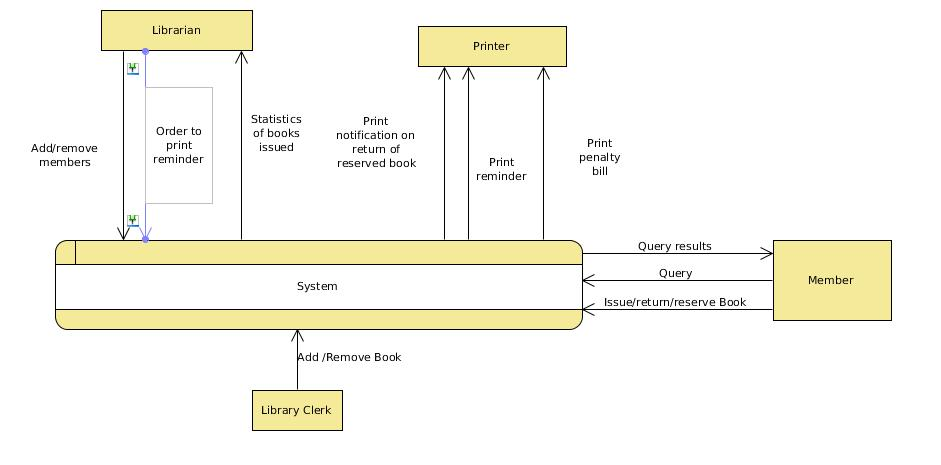
\includegraphics[scale=0.5]{images/contextDiag.jpg}
\item Level 1 DFD\\
\begin{itemize}
\item Diagram for login : \\
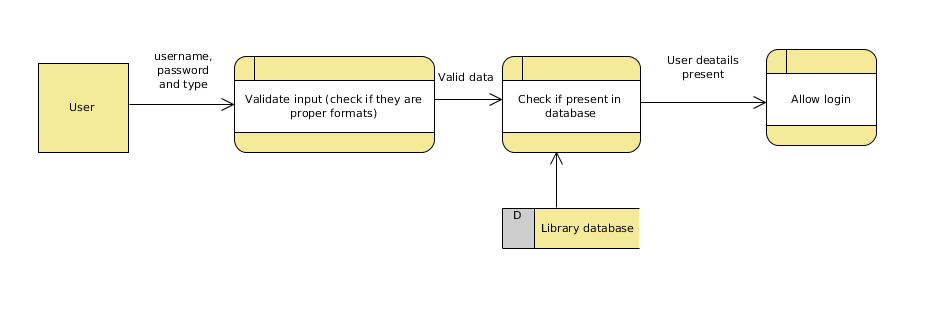
\includegraphics[scale=0.5]{images/dfdDiagLogin.png}\\
\item Diagram for issuing books : \\ 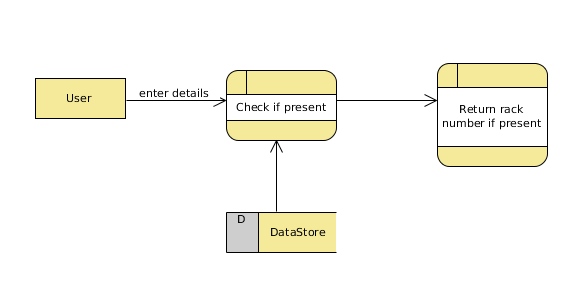
\includegraphics[scale=0.5]{images/DFDDiagIssue.png}\\
\item Diagram for returning books : \\ 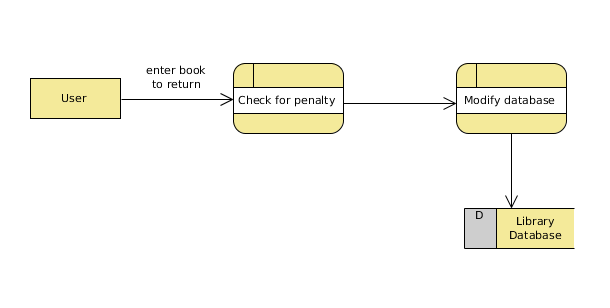
\includegraphics[scale=0.5]{images/dfdDiagReturnBook.png}\\
\item Diagram for searching books : \\ 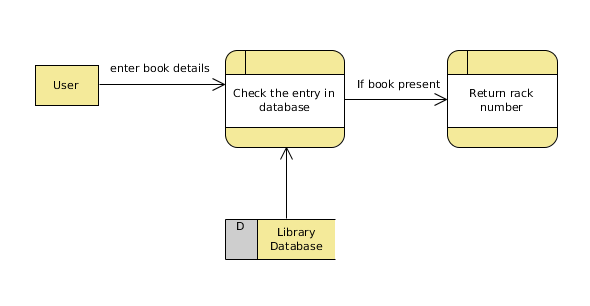
\includegraphics[scale=0.5]{images/dfdDiagSearch.png}\\
\end{itemize}
\end{itemize}



\section{System Parameters}
\subsection{Platform}
The software requires the following platforms to run :
Minimum system requirements :
\begin{itemize}
\item Hardware Requirements :
	\begin {enumerate}
	\item Processor Pentium II processor or higher
	\item Hard Disk space 500MB
	\item RAM 512 MB
	\end{enumerate}
\item Software Requirements :
	\begin{enumerate}
	\item Operating system
		\begin{itemize}
		\item  Windows 7 or later
		\item Linux distributions like Ubuntu 14.04.03 or other
		\end{itemize}
	\item MySQL
	\item Java JDK platform 1.7 or higher
	\end{enumerate}
\end {itemize}
\subsection{Language}
The entire software is written using the language Java.
The object oriented programming paradigm of Java has been followed throughout.
\subsection{Build System}
The code is compiled and built using Java Standard library.Java converts the code into bytecode which is platform independent and can be run onnany system with JRE installed.

\subsection{Libraries}
The libraries used for the software are as follows :

\begin{enumerate}
\item Java Swing (java.awt.*)
\item Java AWT   (javax.swing.*)
\item Java Exception  (java.lang.Exception.*,java.io.*)
\item Java mySQL libraries:(java.sql.*)
\end{enumerate}
\subsection{Sizing}
This is an extremely lightweight software consuming negligibly small amount of main memory during runtime.\\ 
At a later point of time it can be modified to run as a web applet or servlet. 

\subsection{Performance}
Performance of the Library Information of System is enhanced by the following listed technique:
\begin{enumerate}
\item There is practically no lag in the main GUI.This has been ensured by 
ensuring that all cron jobs are run in the background, not hampering the running time of the main GUI.
\item The implementation of database through mySQL considerably speeding up the insertion,deletion and answering queries. mySQL through the use of balanced search trees does all of these in worst case O(lg n) time.This reduces the processing time considerably and speeds up the execution of the software. 

\end{enumerate}
\section{Limitations and Exceptions}
The nnumber of books which can be incorporated into the system has been kept to be constant in this case to ensure a simpler design.
In case of a dynamically ncreasing book set the algorithms and the data structures used to mange have to be optimized further to keep the running time of the software as fast as possible.
\\
Exceptions which are present or handled in this software are as follows :
\begin{enumerate}
\item Username cannot contain any special characters except underscore.Entering any username not following this rule will throw an exception and prompt the user to re-enter the username.
\item The password of the user must be atleast 8 characters long,must constraint atleast one alphabet,atleast one digit and atleat one special character. Violation of these rules will throw an exception and prompt the user to re-enter password.This is done to enhance the security level by making the password extremely difficult to crack by brute force algorithms.
\item The user type by default is empty in the initial  loginscreen.The user must specify the user type while logging in.Keeping it default shall throw an exception and prompt the user to try and login again.
\item The user who has fulfilled his issue/reserve quota may click on issue book.This shall throw an exception and a dialogue box shall appear informing the user to return issued books or cancel reserved books(if any) and then try to issue books.
\item The user who has fulfilled his issue/reserve quota may click on reserve book.This shall throw an exception and a dialogue box shall appear informing the user to return issued books or cancel reserved books(if any) and then try to reserve books.
   
\end{enumerate}
\section{Other Information about analysis}
The other analysis performed are mainly on focusing how to achieve more abstraction and also at the same time maintain the safety and the security of the software
\part{System Design}
\section{Refined System Parameters}
\subsection{Global System Architecture}
The overall system architecture is a 2-tier architecture which includes client at one end and the
database at the other. There is no server based middle tier in the software being designed.
\subsection{Platform}
\subsubsection{Hardware}
The hardware platform required in this software is :
\begin {enumerate}
	\item Processor Pentium II processor or higher
	\item Hard Disk space 500MB
	\item RAM 512 MB
	\end{enumerate}
\subsubsection{Software}
The software platform of the software is fully developed in Java.\\
For suitable execution Java JDK 1.7 or later is required.\\
The database management has been done using a DBMS software like MySQL.\\

\subsubsection{Networking}
The GUI support and the database support are interlinked via a tcp network which facilitates the flow of information between the two ends.It provides scope for dividing the space requirements by distributing the load. The use of tcp network ensures secure data flow between the two interfaces.\\
The tcp network identifies the two ends of the network and establishes a secured connection between the two ends.Keeping the data at a separate location can improve the safety of the software as it prevents data loss to a huge extents in case of a glitch in the GUI end.
\\
Thus we can ensure a safe, secure, reliable and fast software design.\\

\subsection{Software Architecture}
Object-oriented architecture forms the basis of the LIS. In this style data representations and
their associated primitive operations are encapsulated in an abstract data type or object. The components of this style are the objects—or instances of the abstract data types. Objects interact through function and procedure invocations.
Two important aspects of this style are
A. that an object is responsible for preserving the integrity of its representation (usually by
maintaining some invariant over it), and
B. that the representation is hidden from other objects.
Thus the aspects of OOA mentioned justify our choice.
%\subsubsection{Details}
%\subsubsection{Justification}

\section{Database Design}
There is need to maintain a central database to keep all the details of the users and the books in the library to maintain the data more easily.\\
Even though this thing could have been done by using a simple list or even a balanced tree (to increase efficiency) but the use of DBMS is preferred to perform the operation more easily without worrying how the operation is being implemented.\\
Also the DBMS management softwares or the technologies provide very less time complexity to perform all the required operations like adding a record, deleting a record or even searching and modifying a data record which is perfectly applicable for our software.\\
The database used will have the following table : 
\begin{enumerate}
\item \underline{Table of users} :\\
The list or table of all the users/members in the library along with their usernames and passwords which is used for validation of the user.
\item \underline{Table of clerks} : \\
The list or table of all the clerks in the library along with their usernames and password and some other relevant information which may be required in the system.
\item \underline{Table of books} : \\
The table of all the books along with the specification of the copies of the same book present in the library.
\\The fields which needed to be maintained in this table are :
\begin{itemize}
\item the ISBN id or nnumber of the book
\item the name of the book
\item the author of the book
\item nnumber of copies of the same book present in the library
\item the list stating whether any copy of the book is issued
\item the list specifying which user issued which copy
\end{itemize}


Also a backup copy of this entire database needs to maintained to keep the data safety to the maximum level possible.This is to ensure that the data is not lost even if a glitch occurs in the software at any point of time.\\This make the software more user friendly and realistic.
The updation needs to be carried out in both the databases at the same time so that no discrepancy occurs in the tables in both the databases.
\\
\end{enumerate}
\section{Design Details}
The GUI is an interactive environment designed solely in JAVA.The details of the software involves the following steps :
\begin{itemize}
\item User login :
\\The person log into the library system as a regular user or a clerk or as a librarian.Upon successful logging in the user is then directed to his/her respected home page to perform actions of his/her choice.
\item Add a user :
\\The librarian has the opportunity to add a user into the system by entering relevant details.
\item Remove a user :
The librarian also has the opportunity to remove a user from the library database if he/she finds it necessary. Upon doing this all then details of the user is removed from the system.
\item Issue book: 
\\The user can search and issue a book if it is available in the library at that point of time.
\item Reserve book : 
\\The user can also reserve a book if he/she needs it and the book is not available at that point of time at the library.
\\The library system will issue a notification whenever the book is available.
\item Return book : 
\\The user upon successful login will be able to return a book issued earlier.It also checks for the penalty in this stage.

\end{itemize}
\subsection{Refinement of UML diagrams}

\subsubsection{Refinement of Use Case Diagram}

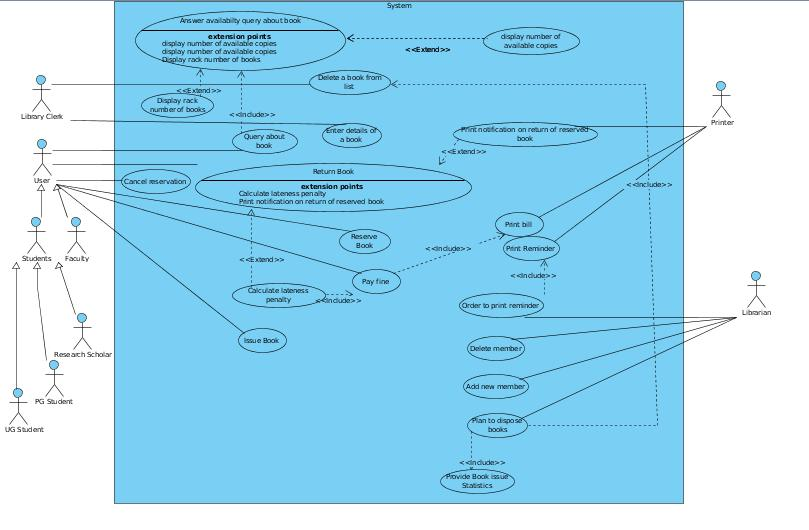
\includegraphics[scale=0.55]{images/useCaseDiag.jpg}\\

\subsubsection*{Use case of User :}
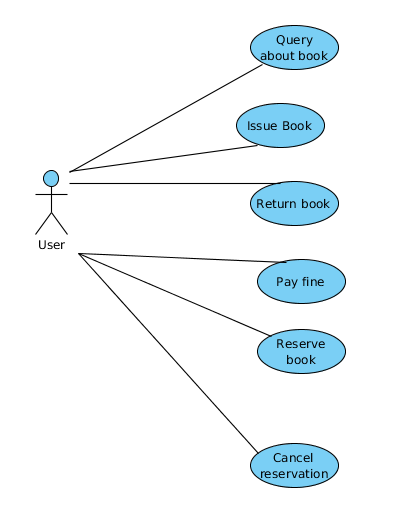
\includegraphics[scale=0.6]{images/userCaseDiag.png}\\
\subsubsection*{Use case of Library Clerk :}
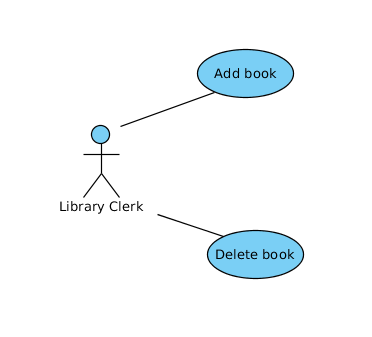
\includegraphics[scale=0.6]{images/clerkClassDiag.png}\\
\subsubsection*{Use case of Librarian :}
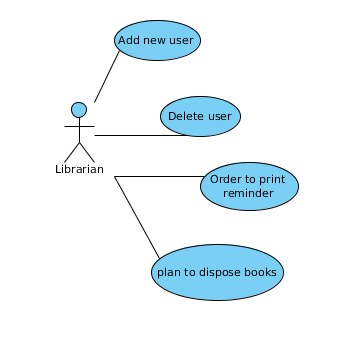
\includegraphics[scale=0.6]{images/librarianCaseDiag.png}\\
Description :
\\
\begin{enumerate}
\item User use cases:
	\begin{itemize}
	
	\item Query about Book\\
	\begin{itemize}
	\item Preconditions:\\
	1. The user must be logged in .\\
	2.The book must exist in the library\\
\item  Postcondition: \\If the book exists in the library,the availablity status of the book is returned\\
 \item Failure Situations:\\ The library does not have  the book \\
 \item Postcondition in case of failure:\\A message to user about the same\\
\item  Actors:\\ User communicates with the system\\
\item  Trigger:\\ User chooses the option to search books\\
 \item Main Success Scenario: \\The library has a copy of the book and it is available for issue.\\
\item  Extensions/Variations: \\The library has a copy of the book but currently none of the copies are available.The book maybe reserved by the user.
	\end{itemize}
 \item Issue Book\\
	\begin{itemize}
	 \item Preconditions:\\
	 1. The user must be logged in .\\
	 2.The book must exist in the library \\
	 3.It must be available for issue.\\
	 4.The user must not have exhausted his quota of nnumber of books\\
 \item Postcondition:\\After successful issue the user account is updated\\
 \item Failure Situations:\\
 1. The library does not have  the book\\ 
 2.The library has the book and it is not available for issue.\\
 3.The user has exhausted his quota of maximum nnumber of books\\
 \item Postcondition in case of failure:\\In failure case 2. the user may choose to reserve the book if he has not exhausted his quota\\
 \item Actors:\\ User communicates with the system\\
 \item Trigger: \\User chooses the option to issue books\\
 \item Main Success Scenario:\\ The library has a copy of the book and it is available for issue.
	\end{itemize}
 

 \item Return Book\\
 \begin{itemize}
 \item Precondition:\\
 1.User must be logged in.\\
 2.User must have previously issued the book.\\
 \item Postcondition:\\
 1.If the book was overdue the penalty is calculated and a bill is printed\\ 
 2.In case the book was reserved by some other user, a notification is sent out to the other user.\\
 3.The user account is updated\\
 \item Failure Situations:\\The user has not issued any book\\
 \item Postcondition in case of failure:\\A message is give to the user about the same\\
 \item Actors:\\ User communicates with the system\\
 \item Trigger:\\ User chooses the option to return issued books\\
\item  Main Success Scenario: \\The user had previously issued the book\\
 \end{itemize}
 
 \item Reserve Book\\
	\begin{itemize}
	\item  Preconditions:\\
	1. The user must be logged in .\\
	2.The book must exist in the library\\ 
	3.It must not  be available for issue.\\
	4.The user must not have exhausted his quota of nnumber of books\\
 \item Postcondition:\\
 1.After successful issue the user account is updated \\
 2.When the book is returned a notification is sent to the user.\\
 \item Failure Situations:\\
 1. The library does not have  the book \\
 2.The library has the book and it is  available for issue.\\
 3.The user has exhausted his quota of maximum nnumber of books\\
 \item Postcondition in case of failure:\\In failure case 2. the user may choose to issue the book if he has not exhausted his quota\\
 \item Actors:\\ User communicates with the system\\
 \item Trigger:\\ User chooses the option to reserve book\\
 \item Main Success Scenario:\\ The library has a copy of the book and it is not available for issue.\\
 
	\end{itemize}
 
 \item Cancel Reservation\\
 \begin{itemize}
 \item  Preconditions:\\
 1. The user must be logged in .\\
 2.The user must have reserved the book\\
 \item Postcondition:\\
 1.After successful issue the user account is updated \\
Failure Situations:\\The user has not issued any book\\
 \item Actors: \\User communicates with the system\\
 \item Trigger:\\ 
 1.User chooses the option to cancel reservation of a book \\
 2.User does not issue the reserved book within 7 days of return\\
 \item Main Success Scenario:\\ The library has a copy of the book and the user must have reserved it previously\\
	
 \end{itemize}

\item Pay Fine\\
	\begin{itemize}
	\item  Precondition:\\
	\begin{enumerate}	
	\item User must be logged in.\\
	\item User must have previously issued the book.\\The book must be overdue\\
	\end{enumerate}
 \item Postcondition:\\
  The book was overdue the penalty is calculated and a bill is printed 
 \item Failure Situations:
 \begin{enumerate}
 \item The user has not issued any book
  \item No returned books are overdue
	\end{enumerate} 
 \item Actors: User communicates with the system
 \item Trigger: User chooses the option to return issued books
 \item Main Success Scenario: The user had previously issued the book and the book is overdue
	\end{itemize}
\end{itemize}


\item Library Clerk Use Cases
 \begin{itemize}
 \item Enter details of a book
 \begin{itemize}
 \item Preconditions:1. The clerk must be logged in.\\2.The book must not be previously entered in the system
 \item Failure Situations:\\ The book is already in the system
 \item Postcondition in case of failure:\\A message to clerk about the same
 \item Actors:\\ library clerk communicates with the system
 \item Trigger:\\ Clerk chooses the option to enter new books
 \item Main Success Scenario:\\ The library  does not have the book and the book is newly entered in the system
\item  Extensions/Variations:\\ The library has the book and the number of copies is increased
\end{itemize}
 \item Delete a book 
 \begin{itemize}
	\item 	Preconditions:\\1. The clerk must be logged in.\\2.The book must  be previously entered in the system \\3.The librarian has decided to dispose the book\\
 \item Failure Situations:\\ The book is not in the system\\
 \item Postcondition in case of failure:\\A message to clerk about the same\\
 \item Actors:\\ library clerk communicates with the system\\
 \item Trigger:\\ Clerk chooses the option to delete books\\
 \item Main Success Scenario:\\ The library  has the book and it is removed from the system.\\
 \item Extensions/Variations: \\The library has the book and the nnumber of copies is reduced.\\
 
\end{itemize}	 
 
 \end{itemize}
 


\item Librarian Use Cases:
\begin{itemize}
 \item Add new member
 \begin{itemize}
  \item Preconditions:1.Librarian must be logged in\\2. A person must apply for membership
 \\ \item Postcondition:\\A new member account is created \\
 \item Failure Situations:\\ The user is already registered\\
 \item Postcondition in case of failure:\\A message to librarian about the same\\
\item  Actors:\\ Librarian communicates with the system\\
 \item Trigger: \\Librarian  chooses the option to add member\\
 \item Main Success Scenario:\\ The user is not previously registered\\
 \end{itemize}

\item Delete member\\ 
 \begin{itemize}
  \item Preconditions:\\ 1.Librarian must be logged in\\ 2. A person must apply for cancellation membership\\ 
 \item Postcondition:\\ The member account is deleted\\ 
 \item Failure Situations: \\ The user has no account\\ 
 \item Postcondition in case of failure:\\ A message to librarian about the same\\ 
 \item Actors: \\ Librarian communicates with the system\\ 
 \item Trigger:\\  Librarian  chooses the option to delete member\\ 
 \item Main Success Scenario:\\  The user   previously has an account\\ 
 \end{itemize}
 
 \item Order to print reminder\\ 
 \begin{itemize}
  \item Preconditions:\\ 1.Librarian must be logged in\\ 2. A book issued by a member must be overdue\\ 
 \item Postcondition:\\ A message is sent to the user.\\ 
 \item Failure Situations:\\  There are no overdue books\\ 
 \item Postcondition in case of failure:\\ A message to librarian about the same\\ 
 \item Actors: \\ Librarian communicates with the system\\ 
 \item Trigger:\\  Librarian  chooses the option to print reminder\\ 
 \item Main Success Scenario :\\  There are some overdue books\\ 
 \end{itemize}

\item Plan to dispose books\\ 
 \begin{itemize}
  \item Preconditions:\\ 1.Librarian must be logged in\\ 2. The book must not have been issued even once for 5 years\\ 
 \item Postcondition:\\ The book is disposed with a message to the library clerk to delete it.\\ 
 \item Actors:\\  Librarian communicates with the system\\ 
 \item Trigger:\\  Librarian  chooses the option to dispose book\\ 
 \item Main Success Scenario:\\  The book has not been issued for 5 years\\ 
 \end{itemize}
 

\end{itemize}

\item System Use Cases:\\ 
 \begin{itemize}
 
  \item Answer availability Query about Book\\ 
	\begin{itemize}
	\item  Preconditions:\\ 1.An user makes a query\\ 
 \item Postcondition: \\ If the book is available, use cases display rack nnumber and nnumber of copies are called\\ 
 \item Actors:\\  System communicates with the user\\ 
 \item Trigger: \\ User chooses the option to search books\\ 
	\end{itemize}

\item Display rack nnumber of book\\ 
	\begin{itemize}
	\item  Preconditions:\\ 1.If the book is available the use case answer availibility query invokes this\\ 
 \item Postcondition:\\  Rack nnumbers are displayed\\ 
 \item Actors:\\  System communicates with the user\\ 
 \item Trigger:\\  answer availibity query triggers this\\ 
	\end{itemize}
 
 \item Display nnumber of copies of book\\ 
	\begin{itemize}
	\item  Preconditions:\\ 1.If the book is available the use case answer availibility query invokes this\\ 
 \item Postcondition:\\  the nnumber of copies of a book are displayed\\ 
 \item Actors: \\ System communicates with the user\\ 
 \item Trigger:\\  answer availibity query triggers this\\ 
	\end{itemize}

\item Calculate lateness penalty\\ 
	\begin{itemize}
	\item  Preconditions:\\ 1.If the book is overdue, return book invokes this\\ 
 \item Postcondition:\\ Penalty is calculated and print bill is invoked\\ 
 \item Actors: \\ System communicates with the user\\ 
 \item Trigger: \\ return book query triggers this\\ 
	\end{itemize}
 
 \item Provide book issue statistics
	\begin{itemize}
	\item  Preconditions:\\ 1.The use case is invoked by plan to dispose books\\ 
 \item Postcondition:\\ Statistics of books is displayed\\ 
 \item Actors: \\ system communicates with librarian\\ 
 \item Trigger:\\ Plan dispose book is invoked\\ 
	\end{itemize}

 \end{itemize}
\item Printer use cases:\\ 
\begin{itemize}
\item Print bill of penalty\\ 
\begin{itemize}
\item Preconditions:\\ Some user must have returned the issued book later than his designated return date.\\ 
 \item Postcondition:\\ Bill of penalty is printed\\ 
 \item Actors:\\  Printer communicates with the system\\ 
 \item Trigger:\\  Calculate lateness penalty triggers print bill\\ 
\end{itemize}

\item Print reminder\\ 
\begin{itemize}
\item  Preconditions:\\ Some user must have exceeded the due date\\ 
 \item Postcondition:\\ Reminder to user is printed\\ 
 \item Actors:\\  Printer communicates with the system\\ 
 \item Trigger:\\ order to print reminder triggers this\\ 
\end{itemize}

\item Print notification on return of reserved book\\ 
\begin{itemize}
\item Preconditions:\\ Some user must have returned a reserved book \\ 
 \item Postcondition:\\ A notification is printed to the user who reserved the book\\ 
 \item Actors: \\ Printer communicates with the system which communicates with user\\ 
 \item Trigger:\\ return book may trigger this use case\\ 
\end{itemize}

\end{itemize}
\end{enumerate}

\subsubsection{Data Flow Diagram}

\begin{itemize}
\item Context Diagram\\
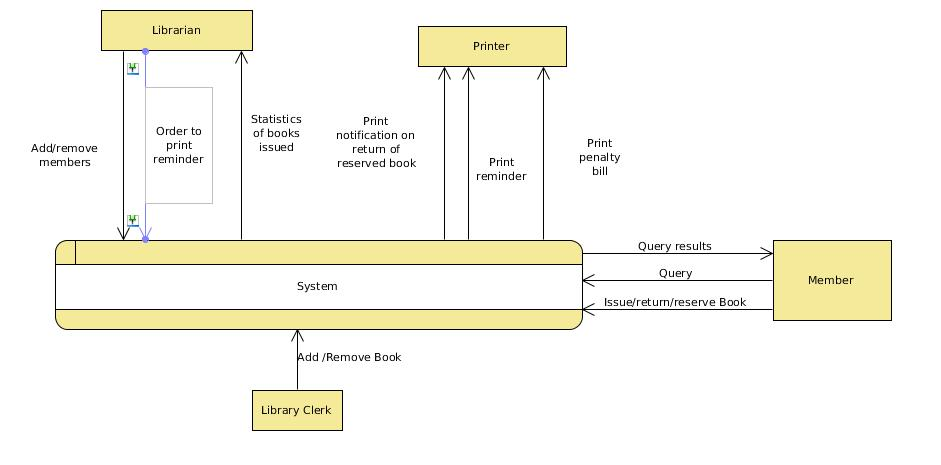
\includegraphics[scale=0.5]{images/contextDiag.jpg}
\item Level 1 DFD\\
\begin{itemize}
\item Diagram for login : \\
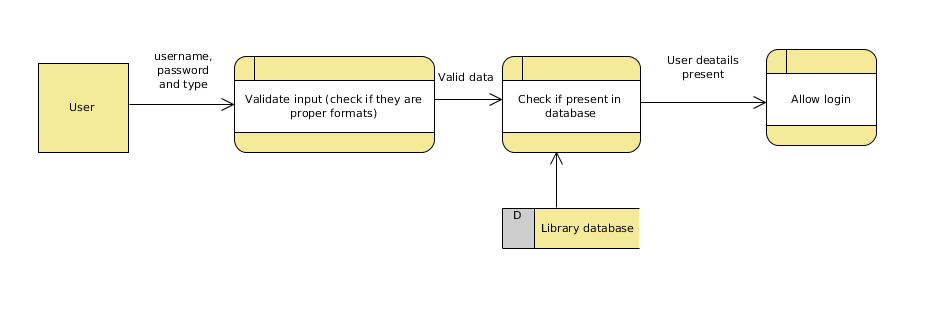
\includegraphics[scale=0.5]{images/dfdDiagLogin.png}\\
\item Diagram for issuing books : \\ 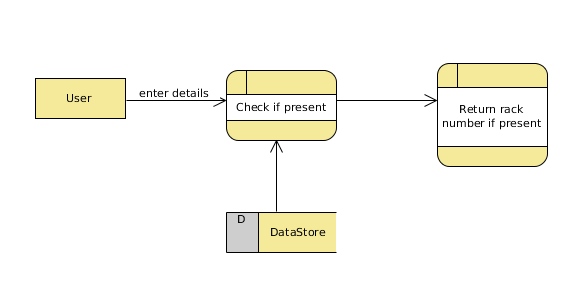
\includegraphics[scale=0.5]{images/DFDDiagIssue.png}\\
\item Diagram for returning books : \\ 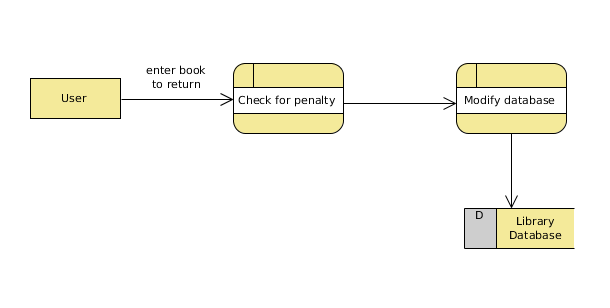
\includegraphics[scale=0.5]{images/dfdDiagReturnBook.png}\\
\item Diagram for searching books : \\ 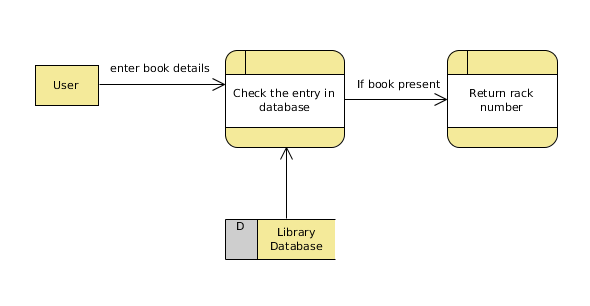
\includegraphics[scale=0.5]{images/dfdDiagSearch.png}\\
\end{itemize}
\end{itemize}
\subsubsection{Refinement of Class Diagrams}
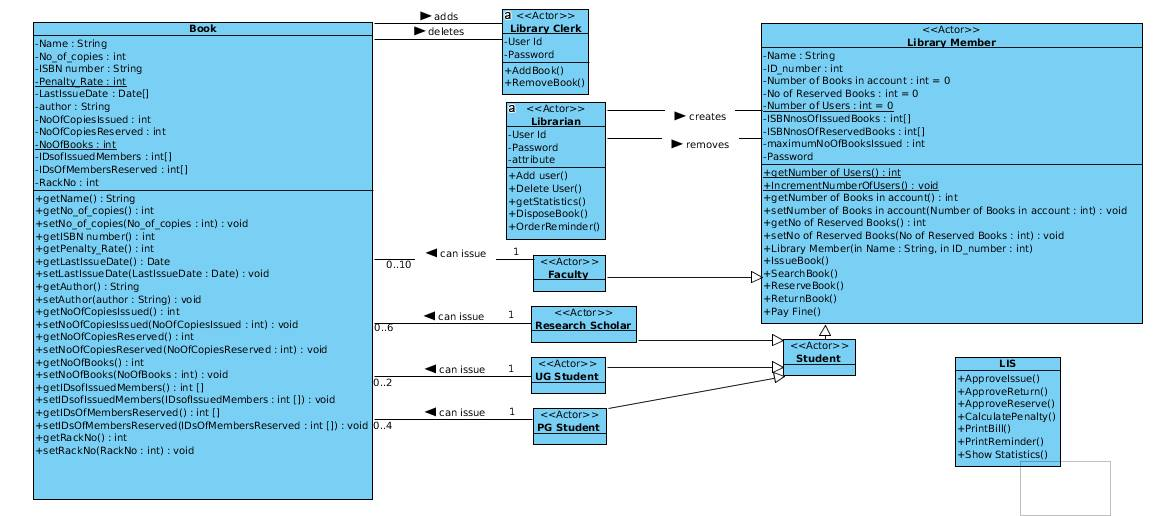
\includegraphics[scale=0.35]{images/classDiagFinal.jpg}
\\
Description of classes:
\\
 \begin{itemize}
\item Book
\begin{itemize}
\item Class Attributes:\\
\\Name:Store the name of book
\\No$\_$of$\_$copies:Stores the nnumber of copies of a book
\\Penalty$\_$Rate:the rate of penalty for book.A static member as it is common for all the books
\\Author:stores name  author of book 
\\LastIssueDateDate:Stores the last issued date of book
\\NoOfCopiesIssued:Stores the nnumber of copies of the book that have been issued out
\\NoOfCopiesReserved:Stores the nnumber of issued books that have been reserved
\\NoOfBooks:A static variable storing the total nnumber of books
\\IDsofIssuedMembers[]:An array of integers storing the ids of all the members who have issued copies of the book
\\IDsOfMembersReserved[]:An array of integers storing the ids of all the members who have issued copies of the book
\\RackNo:stores the rack nnumber where the book is kept

\item Operations:
\\Getter functions for name,No$\_$of$\_$copies,ISBN nnumber,Penalty$\_$rate,LastIssueDate,author,NoOfCopiesIssued,NoOfCopiesReserved,NoOfBooks,IDsofIssuedMembers,IDsOfMembersReserved,RackNo.

We have used getters for these as we need to view these attributes from outside 
\\
Setters for No$\_$of$\_$copies,LastIssueDate,NoOfCopiesIssued,NoOfCopiesReserved,IDsOfIssuedMembers, IDSOfMembersReserved,RackNo.

We have used setters for these as these are changeable with time and need to be changesd at a later point of time.These being private members setters ar only way to modify them
\end{itemize}


\item Library Member 
\begin{itemize}
\item Attributes:
\begin{itemize}
\item Name:Name of the user
\item ID$\_$nnumber:Login id of the user
\item Nnumber of books in account:Total nnumber of issued books
\item Nnumber of reserved books:Total nnumber of books issued by the user
\item NoOfUsers:A static variable storing total nnumber of users
\item ISBNnosOfIssuedBooks[]:an array storing the ISBN nnumber of all books issued by the user
\item ISBNnosOfReservedBooks[]:an array storing the ISBN nnumber of all books reserved by the user
\item maximumNoOfBooksIssued:the maximum nnumber of books that the user can issue
\item password:The login password of the user which is necessary for login authentication
\end{itemize}

\item Operations:
\begin{itemize}

\item Constructor to initialize member\\
\item Getters for NnumberOfBooksinAccount,No ofReservedBooks,NoOfUsers.
We have used getters for these as we need to view these attributes from outside \\\
\item Setters for NnumberOfUsers,Nnumber of books in account,No Of reserved Books.


We have used setters for these as these are changeable with time and need to be changesd at a later point of time.These being private members setters ar only way to modify them
\\
\item IssueBook:called when member tries to issue a book\\
\item SearchBook:Called when member tries to search for a book\\
\item Reserve Book:Called when member tries to reserve a book\\
\item ReturnBook:called when member tries to return a book\\
\item PayFine:Called when member returns an overdue book\\

\end{itemize}
\end{itemize}

\item Library Clerk
\begin{itemize}
\item Attributes:
\begin{itemize}
\item UserId:User Id of the library Clerk\\
\item Password:Password of the library Clerk\\
\end{itemize}

\item Operations:
\begin{itemize}
\item AddBook:Adds a new procured book to database\\
\item Removebook:Deletes a disposed book from database\\
\end{itemize}
\end{itemize}
\item Librarian

\begin{itemize}

\item Attributes:
\begin{itemize}
\item UserId:User Id of the librarian
\item Password:Password of the librarian
\end{itemize}
\item Operations:
\begin{itemize}
\item AddUser:Adds a new user account
\item DeleteUser:Deletes an existing user account
\item getStatistics: asks for statistics from LIS
\item DisposeBooks:Disposes a book not issued in 5 years
\item OrderReminder:Orders LIS to print reminder on overdue books
\end{itemize}
\end{itemize}

\item LIS
\begin{itemize}
\item Operations:\\
\begin{itemize}

\item ApproveIssue:Called when user tries to issue a book
\item ApproveReturn:Called when user tries to return a book

\item ApproveReserve:Called when user tries to reserve a book
\item CalculatePenalty:Calculates penalty on overdue book
\item PrintBill:prints penalty Bill
\item PrintReminder:prints Reminder on overdue books
\item Show Statistics:Display statistics of books issued

\end{itemize}
\end{itemize}

\item Faculty\\
It is a generalization of Library User
\item Student\\
It is a generalization of Library User
\item Research Scholar\\
It is a generalization of Student
\item UG Student\\
It is a generalization of Student
\item PG Student\\
It is a generalization of Student

\end{itemize}
\subsubsection{Sequence Diagram}
\subsubsection*{Add User Sequence Diagram}
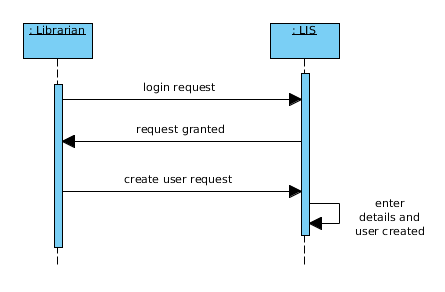
\includegraphics[scale=0.50]{images/seqDiagAddUser.png}
\\
Description : The user needs to login successfully into the account as the librarian as he/she only has the privilege to add a user .He then provides the suitable details required to create a user in the library and creates it.
\\

\subsubsection*{Remove User Sequence Diagram}
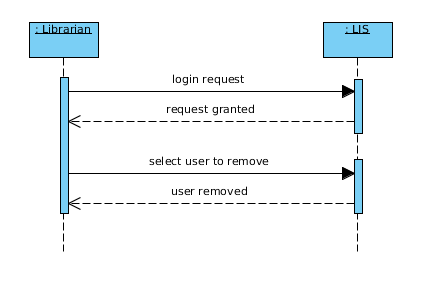
\includegraphics[scale=0.50]{images/seqDiagRemoveUser.png}
\\
Description : The user needs to login successfully into the account as the librarian as he/she only has the privilege to remove a user .He then provides the suitable details required to remove a user in the library and the user along with all the user history is removed from the library database.
\\

\subsubsection*{Add book Sequence Diagram}
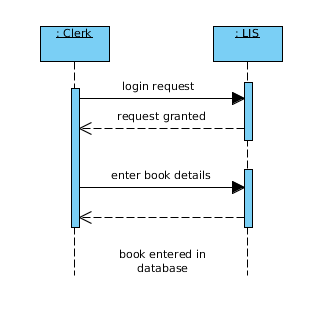
\includegraphics[scale=0.50]{images/seqDiagAddBook.png}
\\
Description : The user needs to login successfully into the account as the library clerk as he/she only has the privilege to add a book into the database of the library.The clerk then provides the suitable details of the book into the system and it automatically updates this into the database at the same time. The book will then be available for issuing ad reservation by the members.
\\

\subsubsection*{Remove book Sequence Diagram}
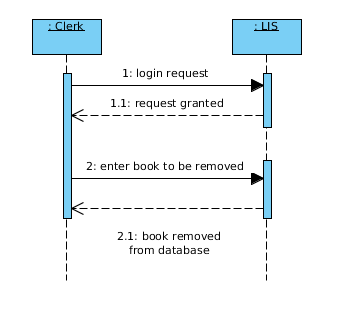
\includegraphics[scale=0.50]{images/seqDiagBookRemoval.png}
\\
The user needs to successfully login as the library clerk as he/she only has the privilege to remove a book from the system if he/she feels that the book has been unused for a long period of time and is not required anymore.The user feeds the details of the book to be removed and the system automatically removes all the records related to this book from the system and will not be thereafter available for issuing and reservation by the other library members/users.
\\

\subsubsection*{Issue book Sequence Diagram}
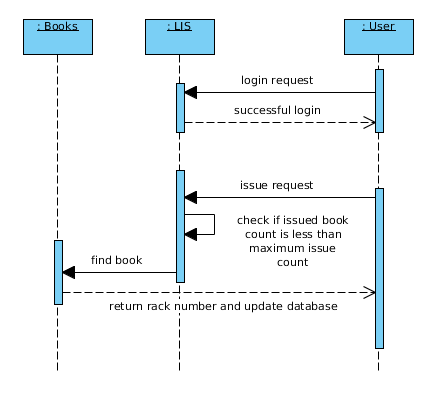
\includegraphics[scale=0.50]{images/seqDiagIssueBook.png}
\\
The user needs to successfully login as a valid member or user of the library to issue a book. Also the book must be available in the library at that instant and also he/she must not exceed the maximum book count against his/her account in the library.The book is then added into the user's account and is thus issued.\\

\subsubsection*{Return book Sequence Diagram}
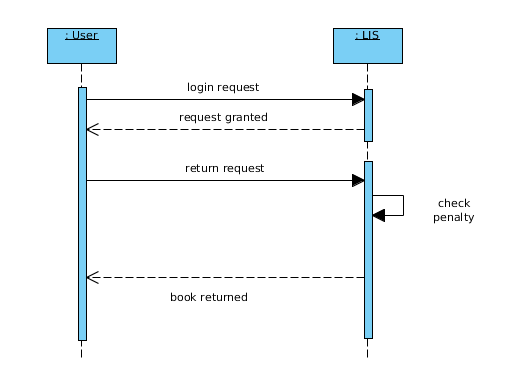
\includegraphics[scale=0.50]{images/seqDiagReturnBook.png}
\\
The user needs to successfully login as a valid member of the library to avail the option of returning the book.The book should not be overdue else the user has to pay a fine as per the rate predecided by the library authority. The book in any case is returned and all changes are updated in the user details of the database.
\\

\subsubsection*{Search book Sequence Diagram}
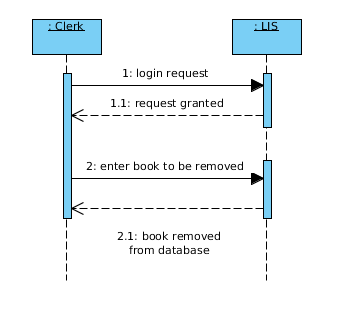
\includegraphics[scale=0.50]{images/seqDiagBookRemoval.png}
\\
The user needs to successfully login to search if a book is present in the library.The user needs to give the details of the book in the system and it will notify about the presence of the book in the library.
\\

\subsubsection{Collaboration Diagram}

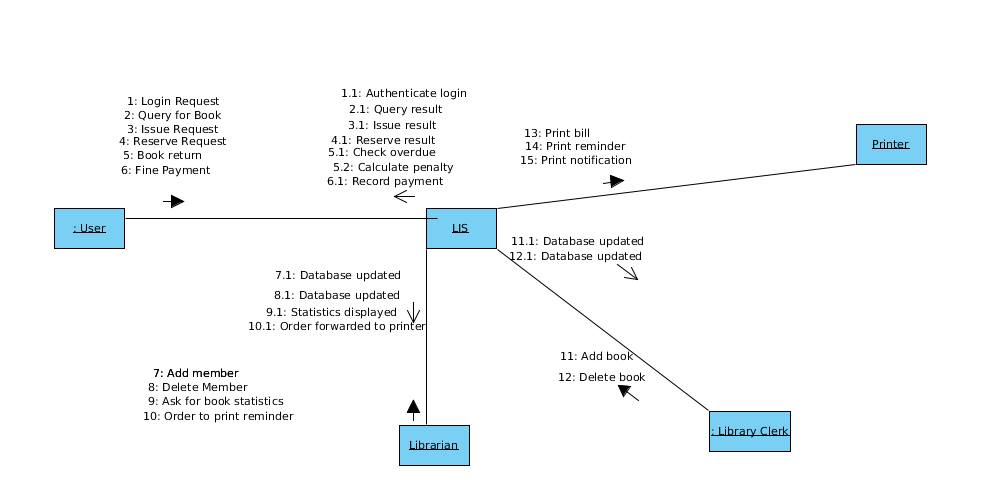
\includegraphics[scale=0.50]{images/collaDiag.jpg}
\\
Description : The user send a specific set of requests to the LIS system like the login request , issue request , return request , search request and penalty/fine payment.The LIS is bound to send back suitable return messages in case of each of the request messages sent ot the system.
\\
The library clerk has the privilege of adding and removing books from the system and the LIS system will automatically update its database inside by a cron job.
\\
The librarian has the sole administrator accesss to the software and the privilege of adding a member as well as removing his record from the library.The librarian can access the user details or the history of any user.He can also take a a look into the statistics of any book that is can see the book history and can send a notification to remove a book to the library clerk in case the book has been unused and unissued for a long period of time.
\\
The printer is also linked with the system and is used to print the notification and the penalty bills and reminder notifications

\subsubsection{Statechart Diagram}

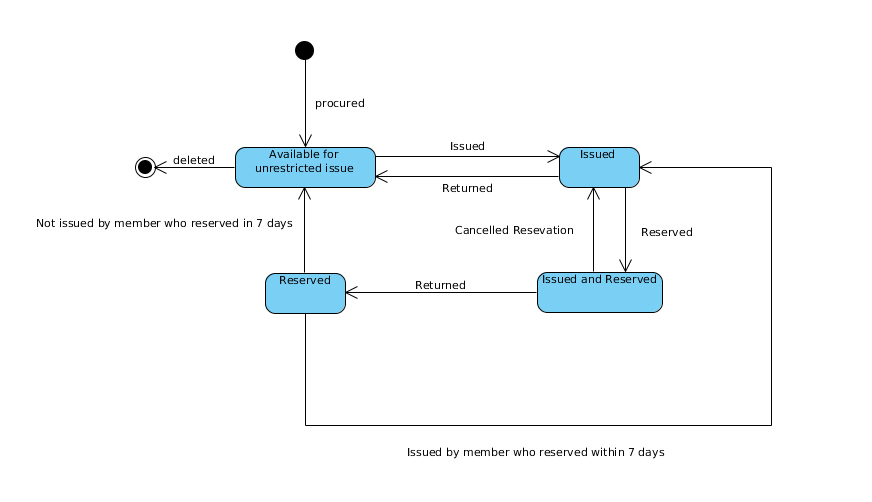
\includegraphics[scale=0.50]{images/stateDiagIssue.png}
\\
Description : The book is avilable for unrestricted issue if it has not been reserved or it has been then the user who has reserved it has not issued it within the 7 days after the notification that the book is available. The book is issued and returned in a separate state. There is also a facility to cancel a reservation .Even after issuing the book may be reserved by some other user. The transition between the states have been clearly shown and demarcated in the above diagram


\subsubsection{Activity Diagram}
\subsubsection*{Issue Book Activity Diagram}
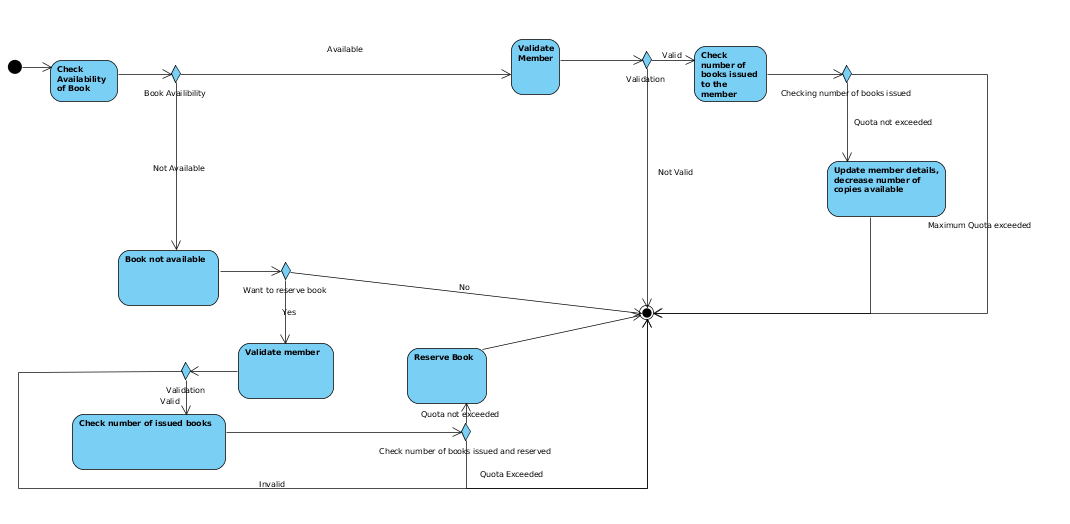
\includegraphics[scale=0.50]{images/activityDiagIssue.png}
\\
Description : First after succesful login the member has to check the availability of the book.We then check if the user is still allowed to issue books or if he has exceeded the maximum book count against his/her account.In case the book is avilable then the book is iisued and the required changes are made to his/her respective account. In case the book is not available then the user can decide to reserve the book or not.If he reserves the book then again we validate him and take a note of the reservation made.A notification will be made to him when the book will be available in the library
\subsubsection*{Return Book Activity Diagram}
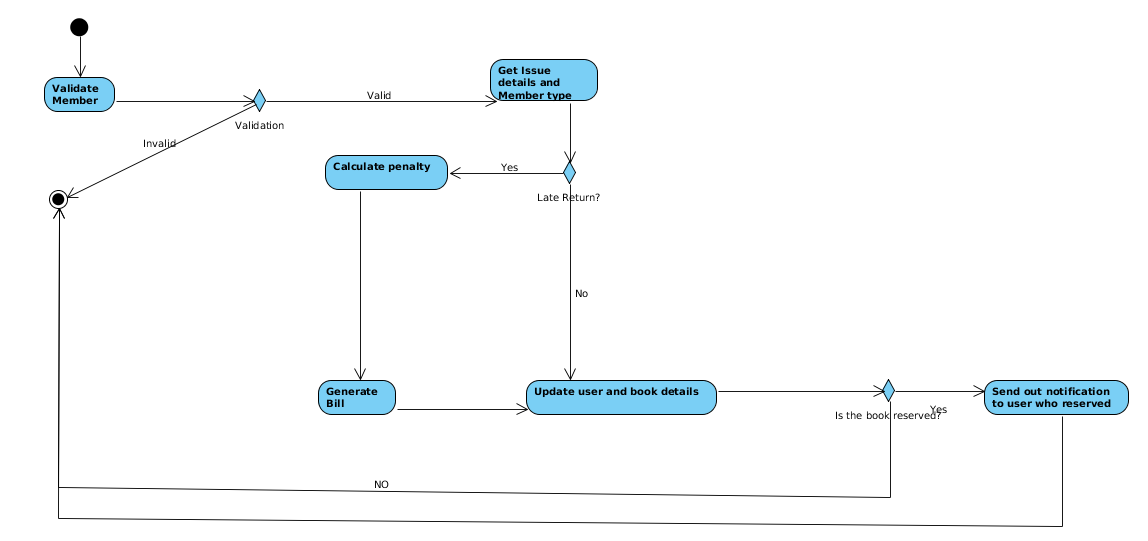
\includegraphics[scale=0.40]{images/activityDiagReturn.png}
\\
Description : We first check for the validation of the member. If the member successfully logs into his/her account then we ask for the book to be returned. The time for the issue is then checked and using that the nnumber of days he book has been kept is calculated. If trhe book has been kept for a longer period of time than it was meant to be the member or the user is liable to pay fines as per the rate predecided.The fine is calculated by a base on the time the book has been overdue.In any case the book is returned and required updation is donw on the account of the user.
\subsubsection*{Search Book Activity Diagram}
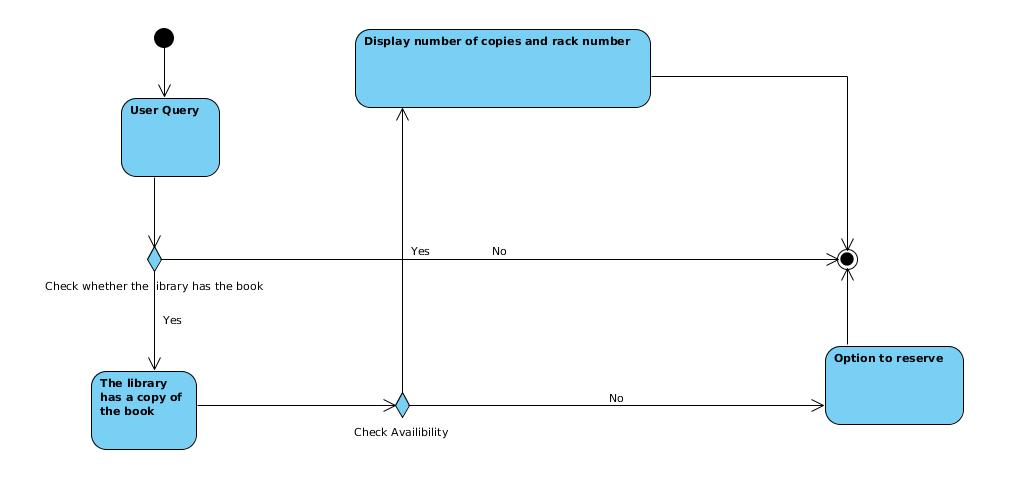
\includegraphics[scale=0.50]{images/activityDiagSearch.jpg}
\\
Description : The user may not need to validate into the system that is the search feature is kept as a global accesss feature. The person needs to put in the details of the book required in the search field to search for its availability. If the book is present the software will display the nnumber of the copies along with their respective rack nnumber for easy accesss else it will display that the book is not currently available.
\subsection{Prototype Design}
The prototype design involves creation of the follwing things :

\subsubsection*{User Login}
Any user with a valid username and password will be able to login to the software to accesss the features. Initially just after the installation of the software only a librarian can be created in the software. Upon thd creation of the librarian the librarian can then create the other users in the library.
\begin{itemize}
\item \underline{For librarian} :\\ If a user logs in as librarian he is then shown a librarian home page screen with the functionalities exclusively of a libraraian.
\item \underline{For clerk} :\\ If user logs in as clerkhe is then shown the clerk home page with the functions like adding or deleting book etc.
\item \underline{For others(members)} : \\We switch on to a new screen which is the home screen of the member. The member has the options of issuing, reserving and returning a book.
\end{itemize}

\subsubsection*{User creation}
The librarian can be created in the beginning when the software is first installed. Once a librarian is creates an new librarian can not be created until and unless the old one is removed.
\\
Only the librarian can create a new member of the library like the faculty or the students.
During the creation of a member the librarian should also provide the type of the user as the maximim book count is different for different categories of the users.Once the type of a library member is given during creation one does not need to provide it anywhere else during issuing or returning of a book as it will be saved in the database and automatically fetched when required.\\
There are several rules while creating the user :
\begin{itemize}
\item The username can consist of alphanumeric characters along with an underscore $(\_)$
\item The password needs to consist atleast one of each type i.e. atleast one alphabet , atleast one nnumber and atleast one special character.\\
The password needs to atleast 8 characters long to ensure good security.
\item The user type also needs to be provided.

\end{itemize}

\subsubsection*{Librarian Home Screen}
The librarian hold the administrator accesss of the library.The feature available to him are as follows :
\begin{itemize}
\item \underline{Creation of user} :\\
For this purpose the librarian will be directed to a new screen where he will have to provide the necessary details in order to create a new account and he has to provide the member type during account creation.
\item \underline{Removing user} : \\
The librarian will provide with the details of the user to remove . If clicked to remove the details of the corresponding user will be removed from the database if and only if all his issued books are returned and there is no penalty due for him.
\item \underline{Print notifications}:\\ The librarian can accesss any user history an can send a request or notification of printing the same
\item \underline{Notification to print penalty bill} :\\ The librarian can send message to the printer to print the penalty bill.
\item \underline{Notification to clerk to remove book} :\\
The librarian can also issue a request to the clerk to remove a book from the kibrary database is he finds it necessary.
\end{itemize}

\subsubsection*{User home screen}
\begin{itemize}
\item \underline{Issue book}:\\
The user can issue book from this portal if the book is present in the library at that point of time.
\item \underline{Return book} :\\ The user can return the book earlier issued via a portal.It also checks if the book is returned in time and if any fine is due.
\item \underline{Reserve book} :\\ The user can reserve any book if it is not present at that point of time and the user will not exceed his maximum issue count.
\item \underline{Search book} :\\ The user can search for any book in the library database by providing any details of the book.If it is present the software will display the rack nnumber of the location of the book.

\end{itemize}
\subsubsection*{Clerk home screen}
\begin{itemize}
\item \underline{Add book} :\\ The clerk can add a book into the library database with all the relevant details
\item \underline{Remove book} :\\ The clerk can remove any old and unused book from the library and remove all its details from the database.
\end{itemize}

\subsection{Design I/O procedures and user interfaces}
The software takes input through a interactive GUI application.\\
Few rudimentary GUI screen of the software have been provided in the section below for showing which are subject to changes as the coding stage progresses.

\begin{itemize}
\item Login Screen : \\
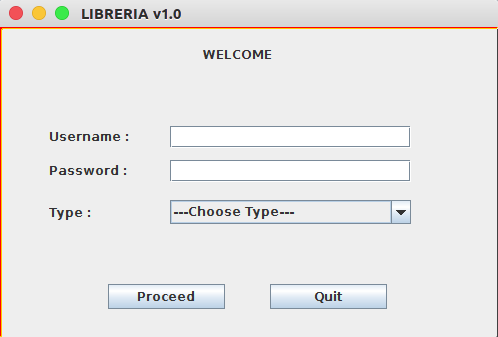
\includegraphics[scale=0.5]{images/login.png}
\item Librarian Home Screen : \\
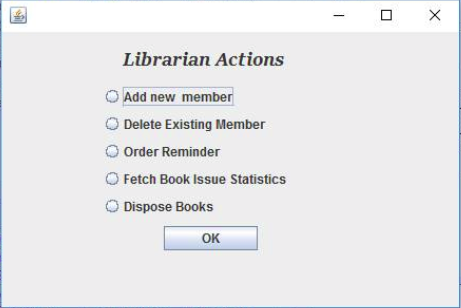
\includegraphics[scale=0.5]{images/librarian.png}
\item Library Clerk Home Screen : \\
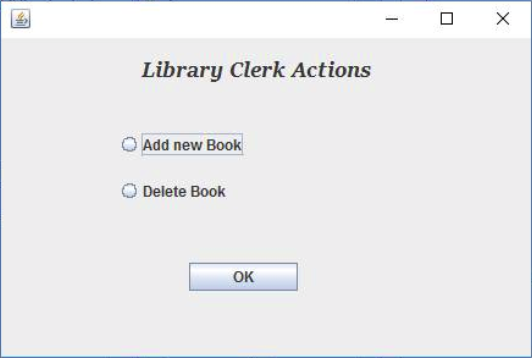
\includegraphics[scale=0.5]{images/clerk.png}
\item Library User Home Screen : \\
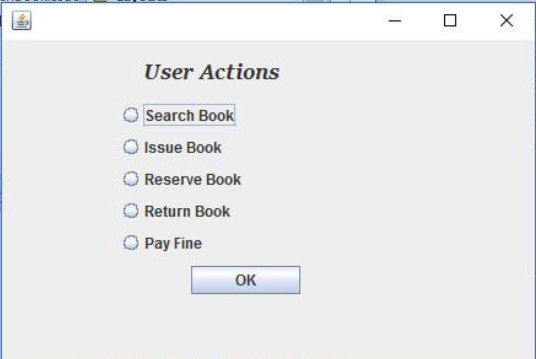
\includegraphics[scale=0.5]{images/user.png}
\end{itemize}

\subsection{Design of classes in target language}
Java being an object oriented language implements classes  as a blueprint or template of objects. Here the main classes shall be books and user.
We shall be using multiple inheritance to classify users into UG students,PG students,Research Scholar and Faculty.
All the data members will be made private to restrict them from being accesssed and modified from outside.Some data members like user id which do need to be accessed outside will have getter functions and setter functions. 

\subsection{Exception Design}
Exceptions which are present or handled in this software are as follows :
\begin{enumerate}
\item Username cannot contain any special characters except underscore.Entering any username not following this rule will throw an exception and prompt the user to re-enter the username.
\item The password of the user must be atleast 8 characters long,must  atleast one alphabet,atleast one digit and atleat one special character. Violation of these rules will throw an exception and prompt the user to re-enter password.This is done to enhance the security level by making the password extremely difficult to crack by brute force algorithms.
\item The user type by default is empty in the initial  loginscreen.The user must specify the user type while logging in.Keeping it default shall throw an exception and prompt the user to try and login again.
\item The user who has fulfilled his issue/reserve quota may click on issue book.This shall throw an exception and a dialogue box shall appear informing the user to return issued books or cancel reserved books(if any) and then try to issue books.
\item The user who has fulfilled his issue/reserve quota may click on reserve book.This shall throw an exception and a dialogue box shall appear informing the user to return issued books or cancel reserved books(if any) and then try to reserve books.
\end{enumerate}
\section{Adoptable Practices}
Some adoptable practices for this software are:
\begin{itemize}
\item Reuse of code from one part to other wherever possible
\item Division of code into small modules for better organization
\item Using camel case and meaningful variable names
\end{itemize}
\section{Any Other Information Of previous Stages}
This is the first release of the software and hence no information about previous stages are
available.
\end{document}
